\documentclass[multi=page, border=0.5cm]{standalone}
\usepackage{calculator}
\usepackage[svgnames]{xcolor}
\usepackage{tikz}

\tikzset{    
    poly/.style={ line width=2mm, red }
}

\definecolor{light-gray}{gray}{0.95}

\begin{document}
\begin{page}
    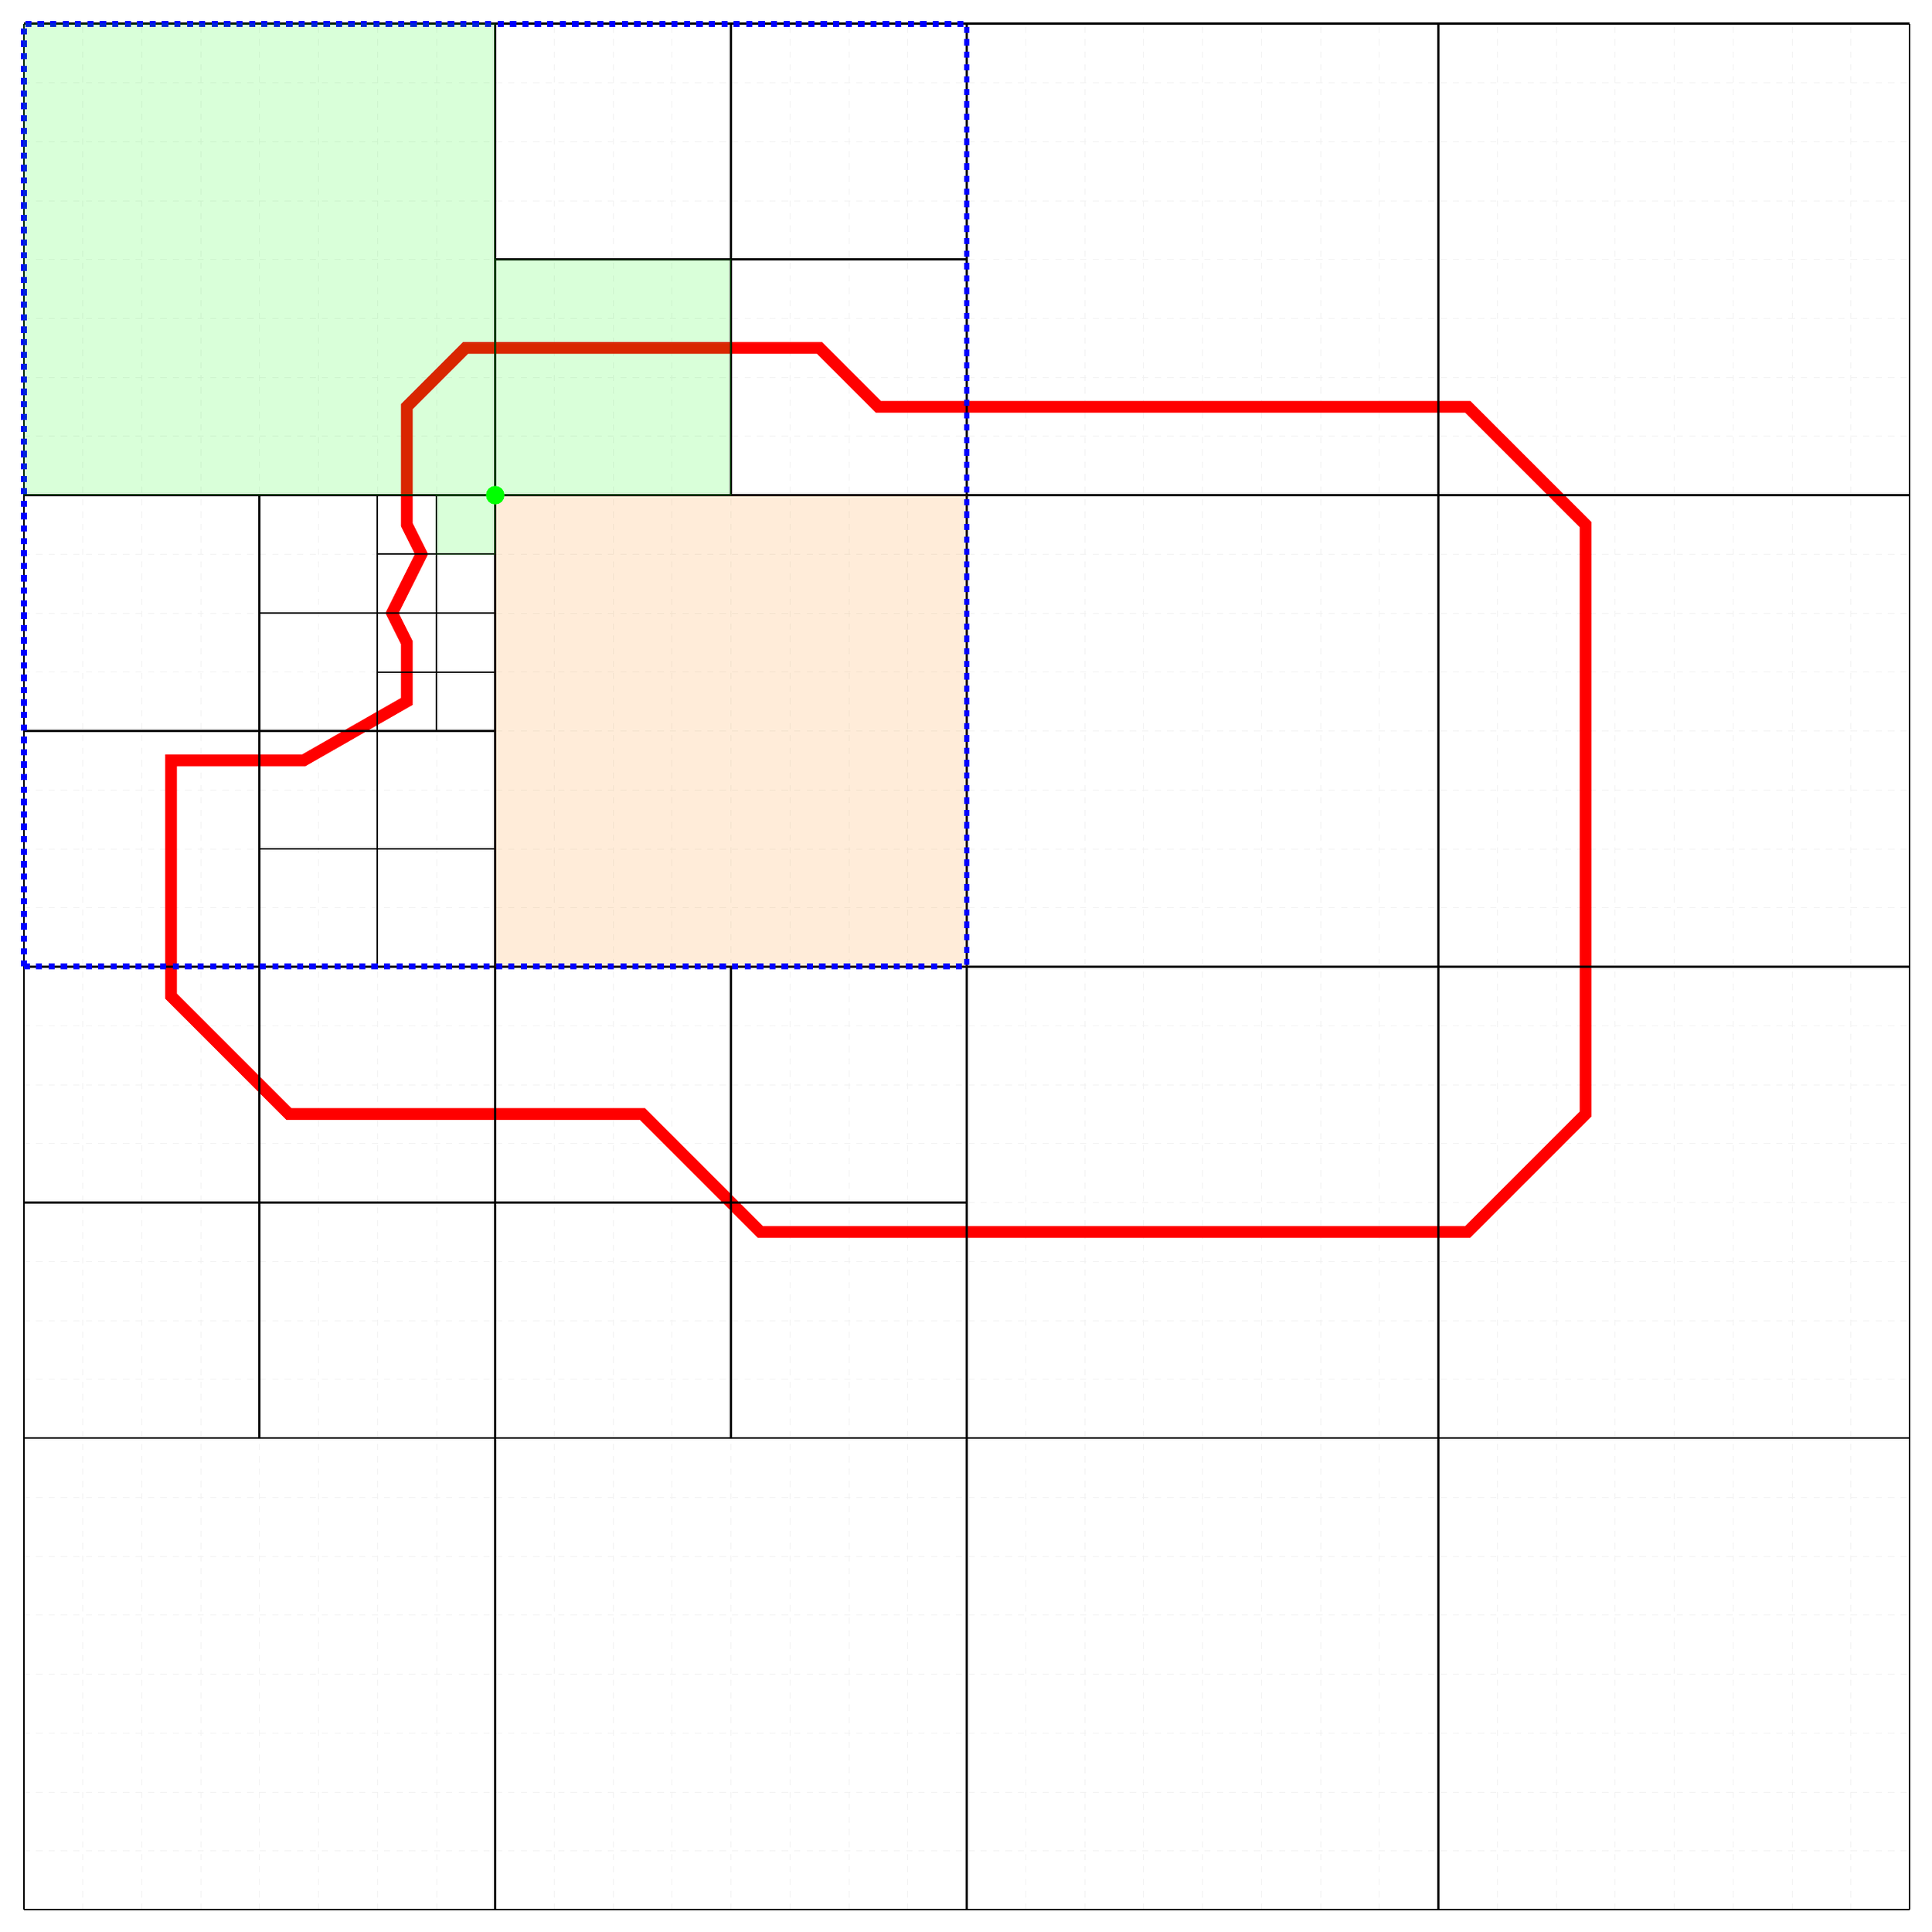
\begin{tikzpicture}
        \draw[step=1, very thin, light-gray, dashed] (0,0) grid (32,32);
        
        \node (start) at (6.50,23.50) {};
        \draw[poly] (start) -- ++(0.25,-0.5) -- ++(-0.25,-0.5) -- ++(-0.25,-0.5)  -- ++(0.25,-0.5)
            -- ++(0,-1) -- ++(-1.75,-1) -- ++(-2.25,0) -- ++(0,-4) -- ++(2,-2)
            -- ++(6,0) -- ++(2,-2) -- ++(12,0) -- ++(2,2) -- ++(0,10) -- ++(-2,2) -- ++(-10,0) -- ++(-1,1) -- ++(-6,0)
            -- ++(-1,-1) -- ++(0,-2) -- (6.75,23);
        \draw[step=8, thick, black] (0,0)  grid (32,32);
        \draw[step=4, thick, black] (0,16) grid (8,24);
        \draw[step=4, thick, black] (0,8)  grid (8,16);
        \draw[step=4, thick, black] (8,8)  grid (16,16);
        \draw[step=4, thick, black] (8,24) grid (16,32);
        \draw[step=2, thick, black] (4,16) grid (8,20);
        \draw[step=2, thick, black] (4,20) grid (8,24);
        \draw[step=1, thick, black] (6,20) grid (8,24);

        \draw[orange, opacity=0.15, fill] (8,16) rectangle (16,24);
        
        \draw[blue, line width=1mm, dashed] (0,16) rectangle (16,32);
        
        \draw[green, fill] (8,24) circle (0.15);
        
        \draw[green, opacity=0.15, fill] (7,23) rectangle (8,24);
        \draw[green, opacity=0.15, fill] (0,24) rectangle (8,32);
        \draw[green, opacity=0.15, fill] (8,24) rectangle (12,28);
    \end{tikzpicture}
\end{page}

\begin{page}
    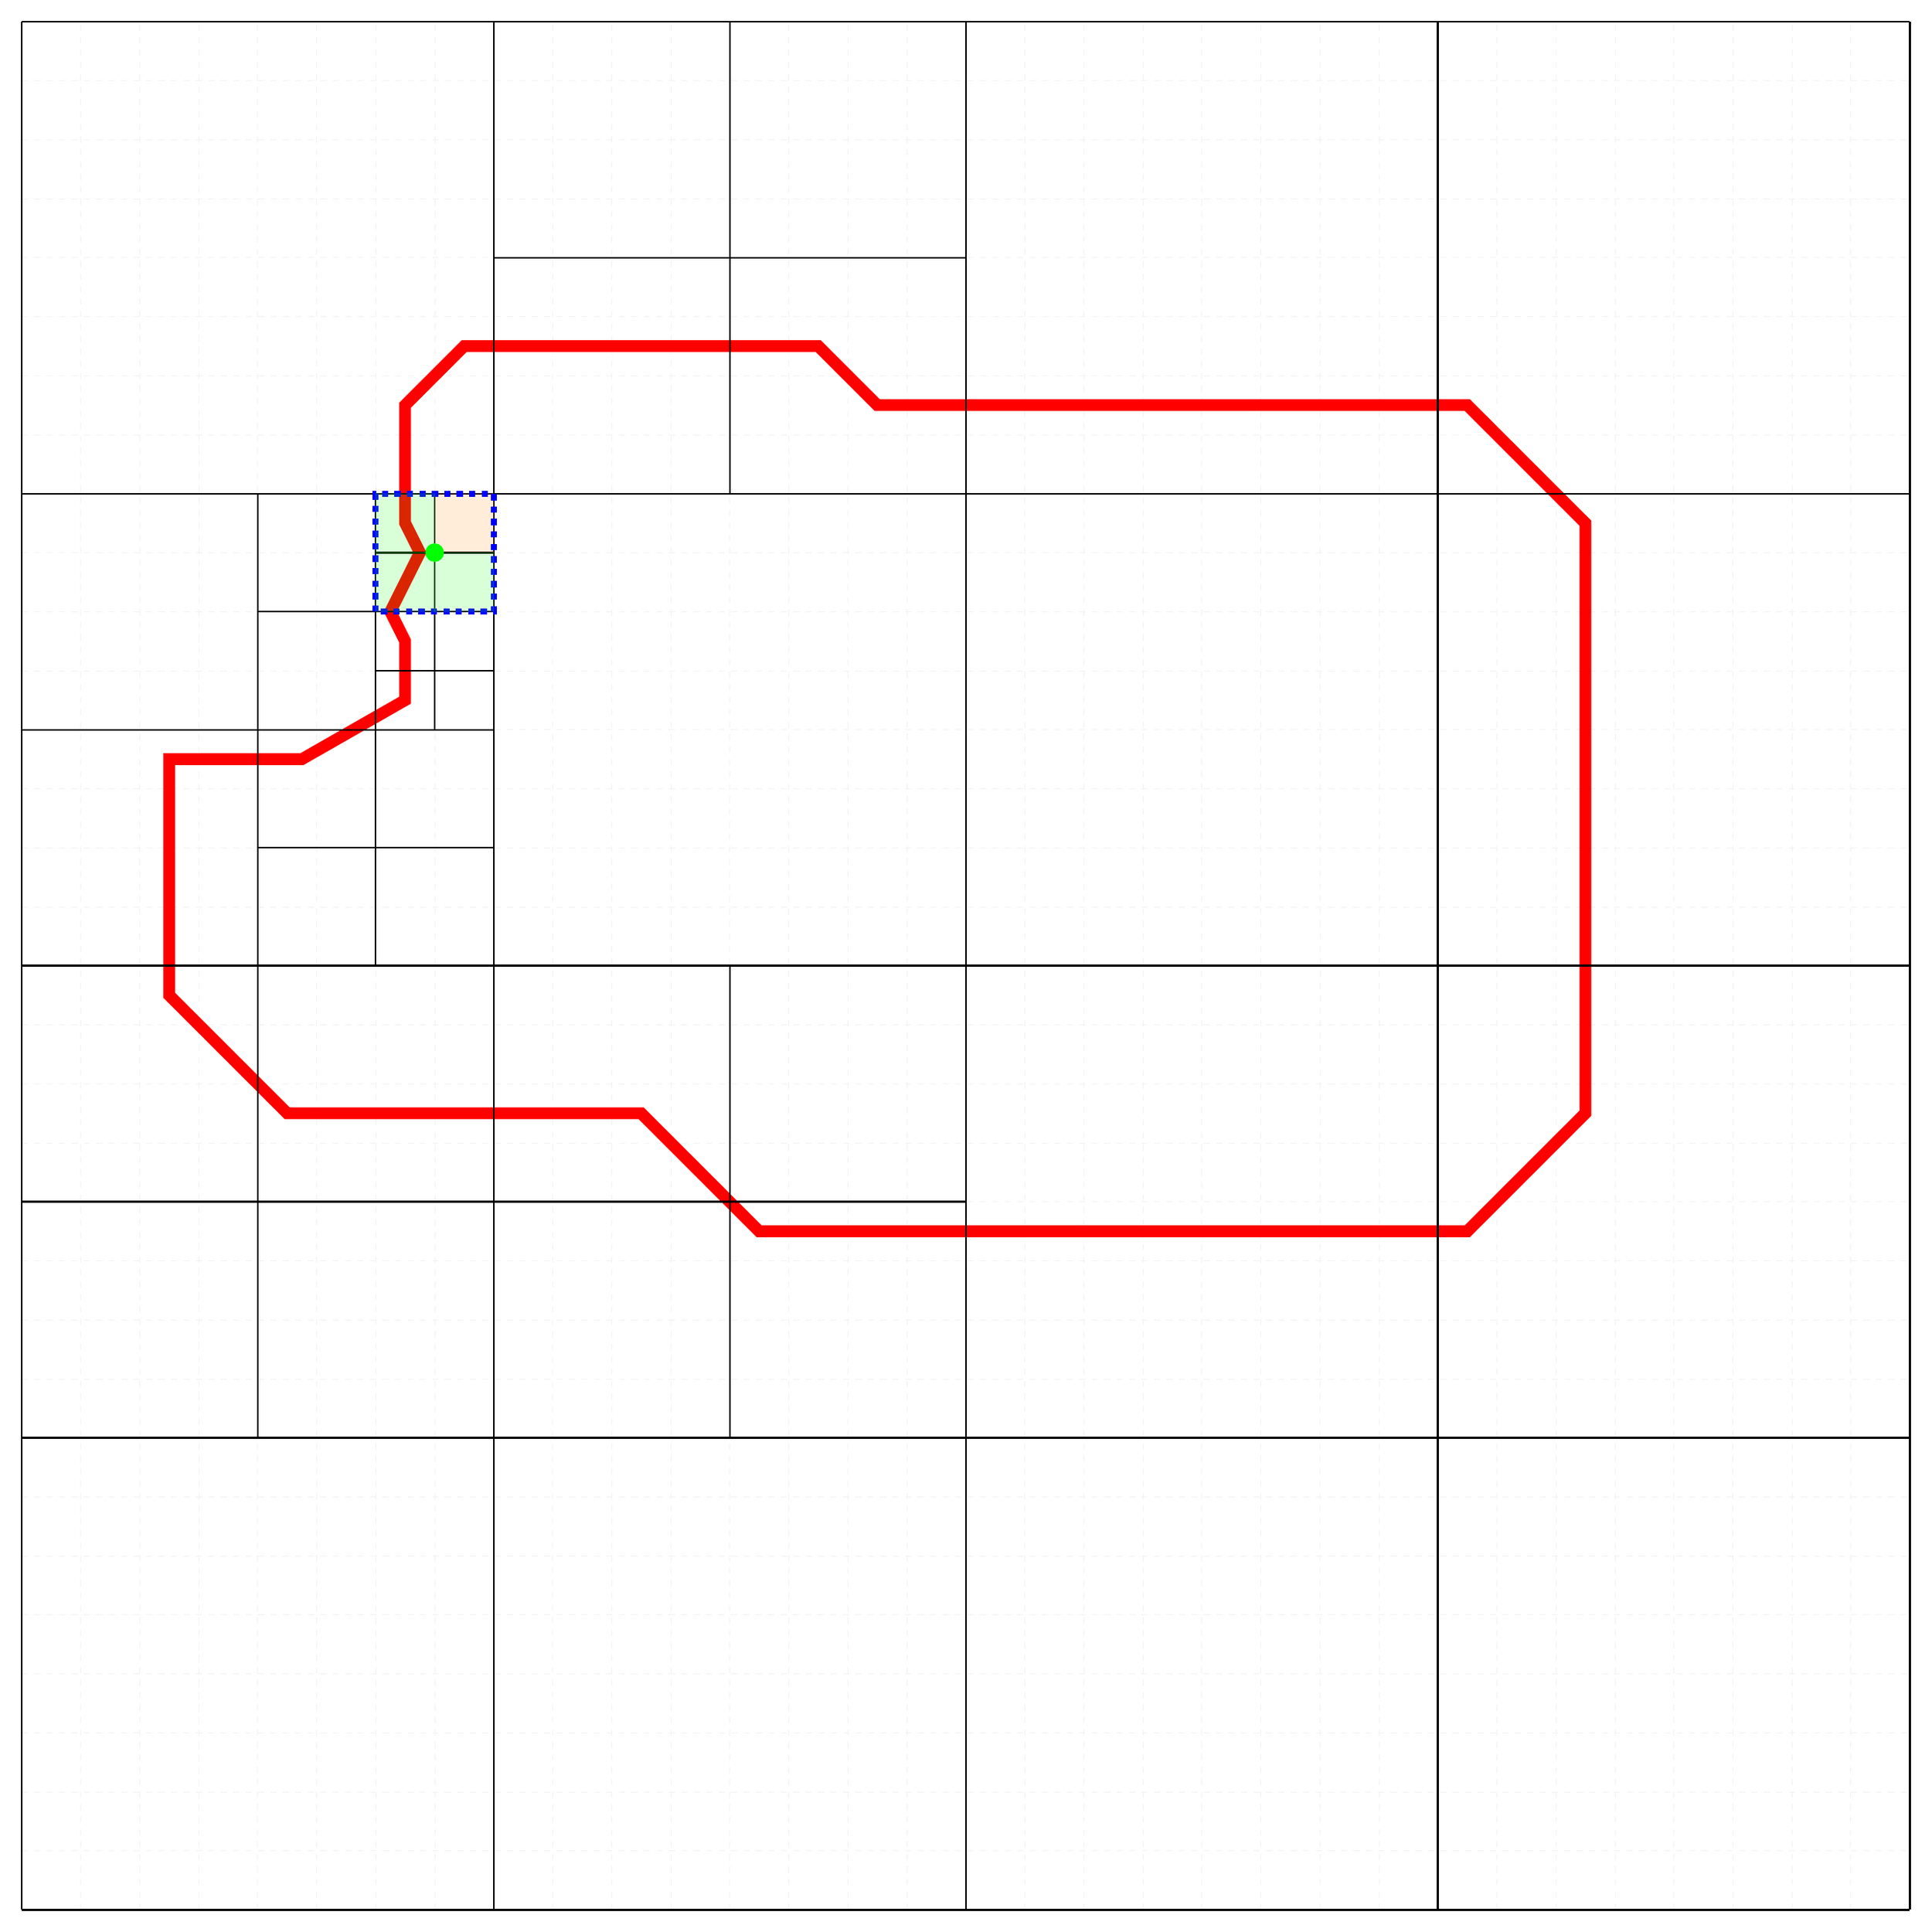
\begin{tikzpicture}
        \draw[step=1, very thin, light-gray, dashed] (0,0) grid (32,32);
        
        \node (start) at (6.50,23.50) {};
        \draw[poly] (start) -- ++(0.25,-0.5) -- ++(-0.25,-0.5) -- ++(-0.25,-0.5)  -- ++(0.25,-0.5)
            -- ++(0,-1) -- ++(-1.75,-1) -- ++(-2.25,0) -- ++(0,-4) -- ++(2,-2)
            -- ++(6,0) -- ++(2,-2) -- ++(12,0) -- ++(2,2) -- ++(0,10) -- ++(-2,2) -- ++(-10,0) -- ++(-1,1) -- ++(-6,0)
            -- ++(-1,-1) -- ++(0,-2) -- (6.75,23);
        \draw[step=8, thick, black] (0,0)  grid (32,32);
        \draw[step=4, thick, black] (0,16) grid (8,24);
        \draw[step=4, thick, black] (0,8)  grid (8,16);
        \draw[step=4, thick, black] (8,8)  grid (16,16);
        \draw[step=4, thick, black] (8,24) grid (16,32);
        \draw[step=2, thick, black] (4,16) grid (8,20);
        \draw[step=2, thick, black] (4,20) grid (8,24);
        \draw[step=1, thick, black] (6,20) grid (8,24);

        \draw[orange, opacity=0.15, fill] (7,23) rectangle (8,24);
        
        \draw[blue, line width=1mm, dashed] (6,22) rectangle (8,24);
        
        \draw[green, opacity=0.15, fill] (6,22) rectangle (7,23);
        \draw[green, opacity=0.15, fill] (7,22) rectangle (8,23);
        \draw[green, opacity=0.15, fill] (6,23) rectangle (7,24);

        \draw[green, fill] (7,23) circle (0.15);
    \end{tikzpicture}
\end{page}
\end{document} 
